\documentclass[11pt,letterpaper]{article}
\usepackage[margin=.72in,top=.73in,bottom=.70in,headheight=15pt,headsep=15pt,footskip=25pt]{geometry}
\usepackage[T1]{fontenc}\usepackage{lmodern}
\usepackage{amsmath,amssymb,tikz,array,fancyhdr,hyperref}
\usetikzlibrary{arrows.meta}
\hypersetup{colorlinks=true,urlcolor=blue}
\renewcommand{\familydefault}{\sfdefault}
\pagestyle{fancy}\fancyhf{}
\fancyhead[L]{\small Week 70 / Shields in a portal room / Adult guide}
\fancyfoot[L]{\scriptsize Bellingham Math Circle / Week 70 / GGT70-FAC-v1}
\fancyfoot[R]{\scriptsize\thepage}
\renewcommand{\headrulewidth}{.3pt}\renewcommand{\footrulewidth}{0pt}
\setlength{\parindent}{0pt}\setlength{\parskip}{7pt}
\newcommand{\sectiontitle}[1]{\par\vspace{4pt}{\large\bfseries #1}\par}
\newcommand{\answer}[1]{\par\vspace{3pt}\textbf{Problem #1.} }
\begin{document}
\sectiontitle{The mathematics first}
\textbf{Exactly four point shields are necessary and sufficient.} In the side-$4$ portal square, $S=(0,0)$ and $T=(2,2)$. Opposite edges are joined by translation: a shot keeps its direction. Every shot that reaches $T$ lifts to a straight segment from the origin to a target copy $(2+4m,2+4n)$, for integers $m,n$.

The midpoint of the segment ending at its \emph{first} target hit folds to one of
\[
(1,1),\quad(1,3),\quad(3,1),\quad(3,3).
\]
These four shields therefore intercept every relevant shot before $T$. Conversely, the four short diagonal paths have disjoint interiors, so no single point can block two of them. Three shields cannot suffice.

\textbf{Assumptions that matter.} A shield is an exact point, never $S$ or $T$; its counter has no blocking radius. Repeated copies represent the same shield. Travel is continuous along straight lines, not restricted to grid roads. Shots stop at their first target hit. A ray that never reaches $T$ is outside the blocking question.

\textbf{What children discover.} Four easy diagonals give a lower bound; unsuccessful shield arrangements lead to a better arrangement; repeated-room pictures turn wraparound into straight lines; finally, a midpoint argument upgrades tests to an all-shot explanation. Testing the finite map is evidence for a conjecture, not its proof.

\textbf{Entry and depth.} This shared Grades 4--5 prototype is for children who can locate grid points, match a point across room copies, and trace a straight line. The final explanation adds halves, even/odd patterns and reasoning about all possibilities. Formal coordinates are optional in a child's explanation. It is not a tested age-placement claim.

\sectiontitle{Set up, launch, and a first route}
\textbf{Per pair:} four small counters, sharp pencil, eraser, straightedge, the four student pages, and spare page 2--3 maps or erasable sleeves. Print at actual size. Mark counter centers; use pencil crosses for their many repeated copies rather than supplying counters for every copy. Keep room edges and grid lines visible. At the older table, two children investigate and the third acts as rotating shot-checker; an adult helps with accurate transfers.

\textbf{Common launch, about 5 minutes.} Let everyone move a counter and trace an edge crossing. Use the printed non-task example: from $(3,1)$, the shot crosses the right seam at $(4,1\frac12)$ and meets the copy $(5,2)$ of shield $P=(1,2)$. In one room it reappears at $(0,1\frac12)$ and reaches $P$. Have children identify the two drawings of one shield, then swap tracer and checker. Do not reveal the four universal positions.

\textbf{Manageable first meeting:} spend roughly 10 minutes on Problem 1, then 10--15 on the four contrasting shots in Problem 2. Use the remaining exploration time on Problem 3 and share one improved arrangement. Stop with a checked four-shield conjecture. Return to Problem 4 when the group wants a guarantee; finishing every page is unnecessary.

\textbf{Rehearse before use.} Check that real counters expose their centers, a ruler can reach the target copies, and children can preserve height at a seam. No physical setup rehearsal or classroom pilot has occurred.
\newpage
\sectiontitle{Answers and optional hints}
\answer{1} The minimum is \textbf{4}. Put one shield strictly inside each corner-to-center diagonal. There are many such arrangements; the four points shown below also solve the later universal problem. All four small student rooms show the \emph{same} arrangement, so put the same four marks in each if recording it on every board.

\begin{center}
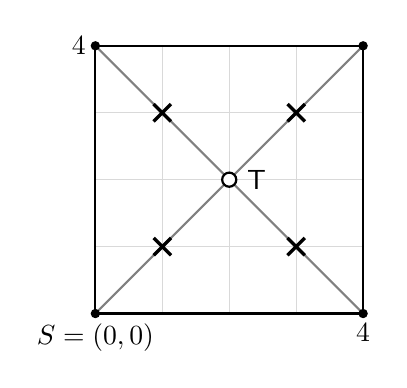
\begin{tikzpicture}[scale=.85]
\draw[step=1,gray!30](0,0)grid(4,4);\draw[thick](0,0)rectangle(4,4);
\foreach\p in{(0,0),(4,0),(0,4),(4,4)}{\draw[gray,thick]\p--(2,2);\fill\p circle(2pt);}
\draw[fill=white,thick](2,2)circle(3pt);\node[right]at(2.12,2){T};
\foreach\x/\y in{1/1,1/3,3/1,3/3}{\draw[very thick](\x-.13,\y-.13)--(\x+.13,\y+.13);\draw[very thick](\x-.13,\y+.13)--(\x+.13,\y-.13);}
\node[below]at(0,0){$S=(0,0)$};\node[below]at(4,0){$4$};\node[left]at(0,4){$4$};
\end{tikzpicture}
\end{center}
\textit{Hint if needed:} ``Where can two of these shots meet before the target?'' Their only shared endpoints are forbidden shield locations. A disk that appears to cover two lines is not a legal point-shield explanation.

\answer{2} The first target depends on the whole segment, not the target name chosen by the shooter.
\begin{center}
\renewcommand{\arraystretch}{1.32}
\begin{tabular}{@{}lll@{}}
Aimed-at copy & First target reached & Halfway shield, folded into room\\\hline
$(2,6)$ & $(2,6)$ & $(1,3)$\\
$(6,2)$ & $(6,2)$ & $(3,1)$\\
$(6,6)$ & $(2,2)$ & $(1,1)$\\
$(10,6)$ & $(10,6)$ & $(1,3)$
\end{tabular}
\end{center}
A simple legal transfer uses $(2,6)$: draw from $(0,0)$ to $(\frac43,4)$, reappear at $(\frac43,0)$, then continue in the same direction to $(2,2)$. The shot to $(6,2)$ is the sideways version. The shot toward $(6,6)$ stops before any portal crossing. The shot to $(10,6)$ crosses right, top, then right before its first $T$.

\textit{Hint if needed:} cover the part of the ruler line beyond the first target. For $(6,6)$, finding a shield halfway to the \emph{chosen} distant copy would be too late. In the table, every midpoint is halfway to the \emph{first} hit.

\answer{3} The four positions $(1,1),(1,3),(3,1),(3,3)$ work. Repeat each mark at the same relative position in every room-copy crossed by a tested line. For example the halfway point toward $(10,6)$ is $(5,3)$, which is the copy of shield $(1,3)$ one room to the right.

The map contains 16 target copies, with each coordinate in $\{-2,2,6,10\}$. Every first-target segment to these copies is intercepted by the arrangement. Let partners pool tests rather than require every child to duplicate every line. A successful finite test does not yet explain shots outside the map.

\textit{Hint sequence:} ``Can your partner find an escaping line?'' Then, if needed, ``Try points at equal fractions along the four short diagonals.'' Reserve ``halfway'' for a pair that wants a stronger hint.
\newpage
\sectiontitle{Why four work for every shot}
\answer{4} The same four shields suffice for arbitrarily long shots. Three can never suffice.

\textbf{Sufficiency.} Unfold the journey only as far as the first target hit. That endpoint is some $(2+4m,2+4n)$, even if it is far outside the printed window. The point halfway there is
\[
\left(\frac{2+4m}{2},\frac{2+4n}{2}\right)=(1+2m,1+2n).
\]
In each coordinate, reducing modulo $4$ leaves either $1$ or $3$. The midpoint is therefore a copy of one of the four shields. It occurs strictly before the target, and cannot be either forbidden endpoint. This proves interception for \emph{every} target-reaching direction, without listing them.

\textbf{A drawing-level explanation.} Each target copy has coordinates $2$ more than a multiple of $4$. Halving either coordinate puts it at an odd grid coordinate. Odd grid points fold to the two positions $1$ and $3$ in each direction, making only four possible halfway locations. Children may show this with doubled strips or several copies before using the formula.

\textbf{Necessity.} Look only at the four shortest shots represented by displacements
\[
(2,2),\quad(2,-2),\quad(-2,2),\quad(-2,-2).
\]
Their open interiors occupy four different quadrants of the room cut at $x=2$ and $y=2$. In the printed room they are the four corner-to-center segments. These interiors never meet, even after identifying opposite edges. A shield away from $S$ and $T$ can lie on at most one. Every one of the four shots needs an interception, so at least four shields are necessary. This lower bound and the midpoint construction agree.

\textit{If the proof stalls:} return to the four short shots for necessity before addressing sufficiency. Ask ``What would one point have to do if there were only three?'' For sufficiency, use a large off-map target chosen by the children and fold its halfway point; then ask what stays unchanged as the copy changes.

\sectiontitle{Use the conclusion carefully}
\textbf{What is established:} the exact minimum for this point-source, point-target portal model. The proof does not concern positive-size obstacles or mirror bounces. Different target/source positions need their own argument; do not carry over the four-diagonal lower bound without checking it.

\textbf{What to notice in a first use:} can children distinguish one shield from its copies, stop at an earlier target, and check a counter's center rather than its edge? Record which representation needed adult help and whether the finite testing game held their interest. These are observations to gather, not results already known.

\sectiontitle{Source and verification}
Samuel Leli\`evre, Thierry Monteil and Barak Weiss, \emph{Everything is illuminated}, \href{https://arxiv.org/pdf/1407.2975}{arXiv:1407.2975}, opening blocking-set definition (p.~1) and Lemma~12(a)--(c) (pp.~12--13). The source gives torus midpoint blocking and blocking cardinality four. The side-$4$ boards, chosen shots and elementary diagonal lower bound here are authored specializations.

The accompanying independent standard-library checker verifies the exact four task rays, all 16 printed target copies, wider finite samples and the launch coordinates. Finite computation supports the printed answers; the arguments above establish the universal claims. This guide matches the four-page GGT70-S-v1 student packet. Digitally checked, unpiloted; physical rehearsal remains outstanding.
\end{document}
